\documentclass[tikz,border=3.14mm]{standalone}
\begin{document}
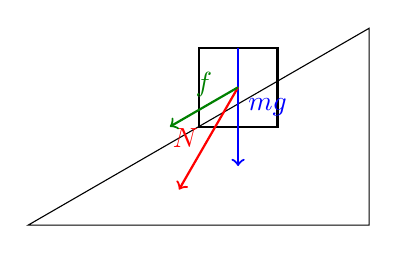
\begin{tikzpicture}

    % Define the angle of the inclined plane
    \def\angle{30}

    % Draw the inclined plane
    \draw (0,0) -- ({5*cos(\angle)}, {5*sin(\angle)}) -- ({5*cos(\angle)}, 0) -- cycle;

    % Draw the block
    \draw[thick] ({2.5*cos(\angle)}, {2.5*sin(\angle)}) rectangle ++(1,1);

    % Draw the forces
    \draw[->,blue,thick] ({2.5*cos(\angle)+0.5}, {2.5*sin(\angle)+1}) -- ++(0, -1.5) node[midway,right] {$mg$};
    \draw[->,red,thick] ({2.5*cos(\angle)+0.5}, {2.5*sin(\angle)+0.5}) -- ++({-90-\angle}:1.5) node[midway,left] {$N$};
    \draw[->,green!50!black,thick] ({2.5*cos(\angle)+0.5}, {2.5*sin(\angle)+0.5}) -- ++({180+\angle}:1) node[midway,above] {$f$};

\end{tikzpicture}
\end{document}